\documentclass[10pt,a4paper]{article}

\usepackage[utf8]{inputenc}
\usepackage[english]{babel}
\usepackage[T1]{fontenc}
\usepackage{amsmath}
\usepackage{amsfonts}
\usepackage{amssymb}
\usepackage{graphicx}
\usepackage{lmodern}
\usepackage{hyperref}
\usepackage[left=2.7cm,right=2.7cm,top=2cm,bottom=3cm]{geometry}
\usepackage{verbatim}
\usepackage{xcolor}
\usepackage{url}

\hypersetup{
    colorlinks,
    linkcolor={red!50!black},
    citecolor={blue!50!black},
    urlcolor={blue!80!black}
}

\title{
\includegraphics[scale=1]{Art/otb-logo.png}\\
  OTB Installation Guide\\
  {\small\url{https://www.orfeo-toolbox.org}}
}

\begin{document}

\maketitle

\tableofcontents

\clearpage
\section{Data package}

The data package for the training can be downloaded at \url{www.orfeo-toolbox.org/packages/WorkshopData/WorkshopData.zip}.

\section{Windows}

\subsection{QGIS}
Install QGIS: \url{http://www.qgis.org/en/site/forusers/download.html}.

\subsection{Command line}
Install a minimal command line environment for Windows. For instance, Git for Windows is very easy to install:
\url{http://git-scm.com/download/win}.

\subsection{OTB and Monteverdi}
To install OTB and Monteverdi, download the appropriate package for your architecture (32 or 64 bits). If you have a 32 bit machine:

\begin{verbatim}
OTB-6.2.0-rc1-Win32.zip
\end{verbatim}

If you have a 64 bit machine:

\begin{verbatim}
OTB-6.2.0-rc1-Win64.zip
\end{verbatim}

These files are available at:
\url{https://www.orfeo-toolbox.org/download/}.
Extract the zip archive in your personal folder, for instance in:\\
\begin{centering}
\texttt{C:{\textbackslash}Users{\textbackslash}John{\textbackslash}install{\textbackslash}}.
\end{centering}

\subsection{Test the installation}
Once the installation is done, OTB applications can be used in several ways. Check that you have a working OTB with the following steps:
\begin{enumerate}

\item Launch \texttt{monteverdi.bat} from the installation folder.

\item Try to open a tif image in Monteverdi (see
figure~\ref{fig:monteverdi}). A demonstration tif image is available here: \url{https://git.orfeo-toolbox.org/otb-data.git/blob/HEAD:/Examples/QB\_Toulouse\_Ortho\_PAN.tif}.

\item The application browser is available from the ``View'' menu 
$\rightarrow$ "OTB-Applications browser".
(see figure \ref{fig:windows-mapla}).

\item Go to the \texttt{bin} folder in the OTB install directory and double-click on the \texttt{.bat} file corresponding to the application to be run, for instance:\\
\texttt{John{\textbackslash}install{\textbackslash}OTB-6.2.0-rc1-win32{\textbackslash}bin{\textbackslash}otbgui\_Rescale.bat}
(see figure \ref{fig:windows-otbgui}).

\end{enumerate}

\begin{figure}[h]
  \center
  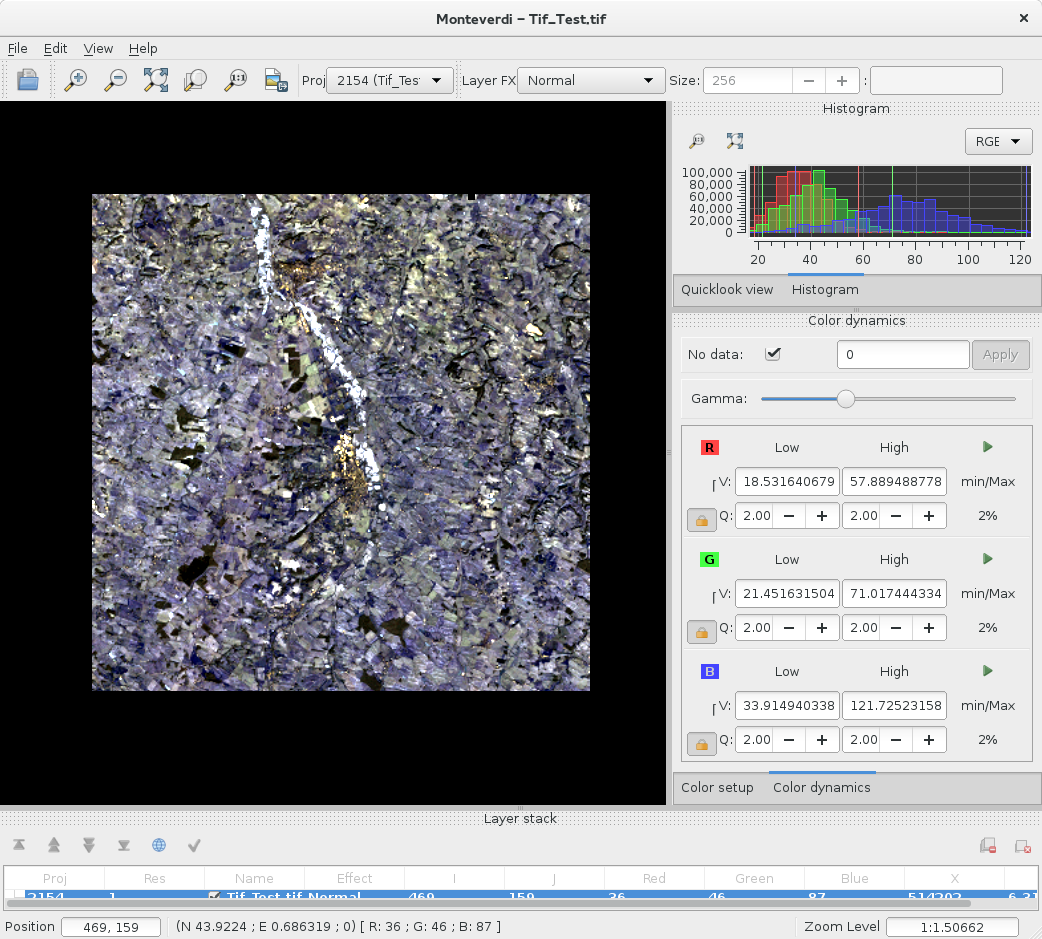
\includegraphics[width=1\textwidth]{Art/monteverdi-tif.png}
  \caption[]{Monteverdi}
  \label{fig:monteverdi}
\end{figure}

\begin{figure}[h]
  \center
  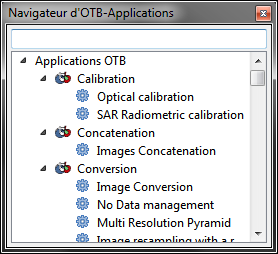
\includegraphics[scale=1]{Art/windows-mapla.png}
  \caption[]{OTB applications can be used from Monteverdi}
  \label{fig:windows-mapla}
\end{figure}

\begin{figure}[h]
  \center
  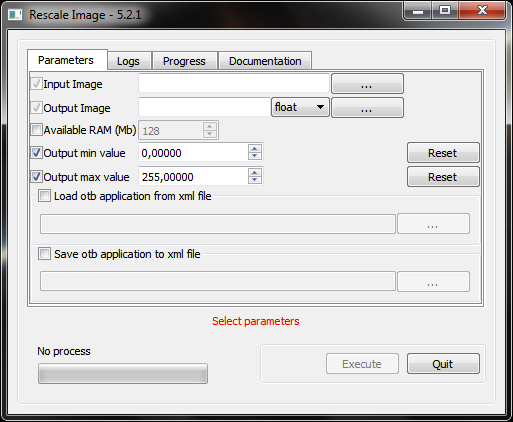
\includegraphics[scale=1]{Art/windows-otbgui.png}
  \caption[]{OTB Graphical User Interface}
  \label{fig:windows-otbgui}
\end{figure}

% En commentaire pour l'instant, c'est peut être un peu inutile puisqu'il n'y a
% aucune action associée en terme d'installation
\begin{comment}
\subsection{OTB in QGIS}

OTB applications are available in QGIS.

Warning ! OTB version distributed with QGIS is sometimes different than the last
stable version.

Eventually you can replace the OTB version used inside QGIS. You'll have to
update the provider option in the QGIS processing properties. 

\begin{figure}[h]
  \center
  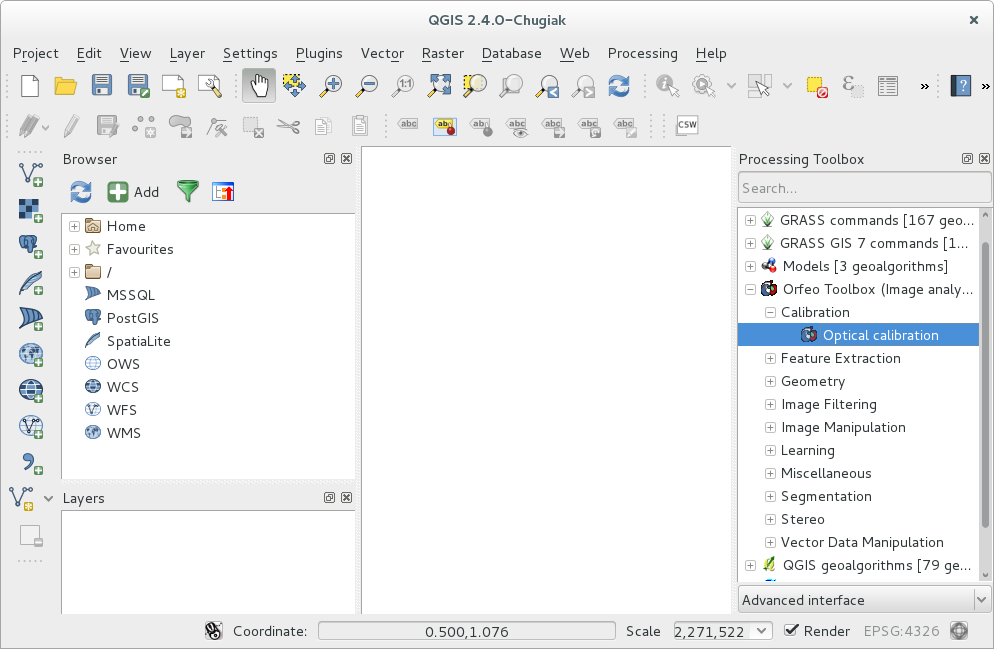
\includegraphics[width=1\textwidth]{Art/qgis-otb.png}
  \caption[]{OTB in QGIS}
  \label{fig:otb-qgis}
\end{figure}
\end{comment}

\clearpage
\section{Linux (Ubuntu example)}

This section explains how to install the tools in a Linux environment like Ubuntu. This procedure can also be used on other Linux distributions by using the appropriate package manager (dnf, yum,
emerge, pacman\ldots)

\subsection{QGIS}
QGIS can be installed via a command line like:
\begin{verbatim}
sudo apt-get install qgis
\end{verbatim}

\subsection{Dependencies installation}
Before installing the self-extracting Linux binary for OTB, several system dependencies have to be installed. In a terminal, type the following:
\begin{verbatim}
sudo apt-get install libx11-6 libxext6 libxau6 libxxf86vm1 libxdmcp6 libdrm2
\end{verbatim}
or the equivalent for other distributions.

You will need the libgl1 and libglu1 libraries, which have different implementations (MESA, FGLRX, NVIDIA, etc.). If you don't already have these libraries, you can use the MESA implementation:
\begin{verbatim}
sudo apt-get install libgl1-mesa-glx libglu1-mesa
\end{verbatim}

\subsection{Install OTB and Monteverdi}
Download the self-extracting binary for Linux (64 bits), available at:
\begin{center}
\url{https://www.orfeo-toolbox.org/download}
\end{center}

The self-extracting binary will extract itself in the current directory. First, the archive has to be made executable, and then it can be run:
\begin{verbatim}
chmod +x OTB-6.2.0-rc1-Linux64.run
./OTB-6.2.0-rc1-Linux64.run
\end{verbatim}

The executable binaries will be inside the 'bin' directory, and you can put this directory in your PATH variable if you want to. 

There are also scripts which set all the environment variables to allow to run Monteverdi and Mapla:
\begin{verbatim}
cd OTB-6.2.0-rc1-Linux64
./monteverdi.sh
./mapla.sh
\end{verbatim}

\subsection{Test the installation}
Once the installation is done, OTB applications can be run in several ways. Check that you have a working installation with the following steps:
\begin{enumerate}

\item Try to open a tif image in Monteverdi (see
figure~\ref{fig:monteverdi}). A demonstration tif image is available here: \url{https://git.orfeo-toolbox.org/otb-data.git/blob/HEAD:/Examples/QB\_Toulouse\_Ortho\_PAN.tif}.

\item The application browser is available from the ``View'' menu 
$\rightarrow$ "OTB-Applications browser".
(see figure \ref{fig:windows-mapla}).

\item Run an application using the terminal, for instance
\texttt{otbgui\_Rescale}. (see figure \ref{fig:windows-otbgui}).

\end{enumerate}

\clearpage
\section{Mac OS X}

The software can also be installed on Mac OS X.

First install QGIS using the instructions for Mac OS X on the official site. To install OTB and  Monteverdi download 
OTB-6.2.0-rc1-Darwin64.run from \url{https://www.orfeo-toolbox.org/download/}.

This is a self-extracting binary which extracts itself in the current directory. Testing the installation is done like in the Linux case.


\clearpage
\section{Python install for OTB}

Starting from OTB 5.8.0, OTB bindings for Python 2.7 are distributed with binary package. With OTB 6.4.0, additional bindings for Python 3.5 are also included. Please note that using a different Python version may not be compatible with OTB wrappings. If no compatible Python 2.x version is found a notification is generated during the installation process. If the installation completes without issue, information relating to your Python bindings will be provided.

You must have Python numpy bindings installed in your system. They can be installed locally without admin rights as follows: “pip install –user numpy”. This is to give users the option to select their own existing Python installation rather than the one dibstributed by the OTB package.

By default, bindings for Python 2.7 will be enabled with the otbenv script. If you want to use bindings for Python 3.5, you can copy this script and modify:
\begin{verbatim}
lib/python into lib/python3, for variable PYTHONPATH
\end{verbatim}

Notes:
\begin{enumerate}

\item You must use monteverdi and mapla through mapla.sh and monteverdi.sh helper scripts in extracted directory.
\item The helper scripts for monteverdi and mapla set required environment variables
\item You might be tempted to move “OTB-6.4.0-Linux64” into another location say /usr/local/ after extraction. But avoid this action!
\item To have “OTB-6.4.0-Linux64” installed in /usr/local or /opt execute “OTB-6.4.0-Linux64.run” in that directory.
\item Multiple installation of OTB can exists in same system without one conflicting the other!

\end{enumerate}

\subsection{Test}
In order to test the Python OTB dependencies, try:
\begin{enumerate}
\item Launch the python console (Linux: ./python ; Windows: python.exe)
\item Try: import numpy
\item Try: import otbApplication
If no error message is printed, everything is fine. If not, check the Python version (2.7 or 3.5), and the PATH and PYTHONPATH variables.
\end{document}
